\chapter{De levende bodem}\label{ch:b2:living-soil}

Het laatste boek van Charles Darwin, verschenen een jaar voor zijn dood, ging
over regenwormen. Hij had in 1842 op een veld bij zijn huis een krijtmarkering
gelegd en die in 1871 opgegraven: ze lag achttien centimeter diep, begraven
onder de uitwerpselen die de wormen naar het oppervlak hadden gebracht, in een
tempo dat hij mat, woog en vermenigvuldigde --- tien ton aarde per acre per
jaar die door hun lichamen ging, zodat ``de hele oppervlakkige teellaag over
zo'n oppervlak om de paar jaar door de lichamen van wormen is gegaan en weer
zal gaan.'' De \omterm{def:b2:living-soil:soil}{bodem} is met andere woorden geen ondergrond waarop levende wezens
staan, maar iets wat levende wezens maken. Dit hoofdstuk gaat over dat maken:
hoe gesteente \omterm{def:b2:living-soil:soil}{bodem} wordt en hoe traag, wie erin leeft en in welke aantallen,
hoe dood materiaal uit elkaar wordt gehaald en wat er overblijft, hoe de wortels
van planten met schimmels en bacteriën onderhandelen over wat ze alleen niet
kunnen krijgen, en hoe snel een \omterm{def:b2:living-soil:soil}{bodem} die tienduizend jaar nodig had om te
ontstaan, verloren kan gaan.

\section{Wat bodem is}

\begin{definition}[Bodem en zijn horizonten]\label{def:b2:living-soil:soil}
\index{bodem}\index{bodemhorizont}\index{humus}\index{verwering}\index{bodemvorming}
\emph{Bodem} is de laag van verweerd mineraal materiaal, organisch
materiaal, water, lucht en organismen die het land bedekt en planten draagt:
ongeveer de helft van zijn volume bestaat uit poriën, gevuld met water of lucht
in wisselende verhouding, en de vaste helft uit minerale korrels ---
zand (\qtyrange{0.05}{2}{mm}), silt (\qtyrange{2}{50}{\micro m}) en
klei (onder \qty{2}{\micro m}), waarvan de verhoudingen de
\emph{textuur} bepalen --- met enkele procenten organisch materiaal dat de
meeste eigenschappen ervan bepaalt. Een bodemprofiel toont
\emph{horizonten}: de \emph{O}-horizont van strooisel en gedeeltelijk vergaan
organisch materiaal aan het oppervlak; de donkere \emph{A}-horizont van minerale
bodem vermengd met \emph{humus}, het stabiele, donkere, colloïdale residu van
de afbraak; de \emph{B}-horizont daaronder, waarin klei, ijzer en opgeloste
stoffen worden ingespoeld en zich ophopen; de \emph{C}-horizont van verweerd
moedergesteente; en het vaste gesteente. Een bodem ontstaat
(\emph{bodemvorming}) door vijf factoren --- moedermateriaal, klimaat,
organismen, reliëf en tijd --- en hij ontstaat traag: verwering levert in de
orde van \qty{0.1}{mm} bodem per jaar op, zodat een meter bodem tienduizend
jaar werk is.
\end{definition}

\begin{omfigure}
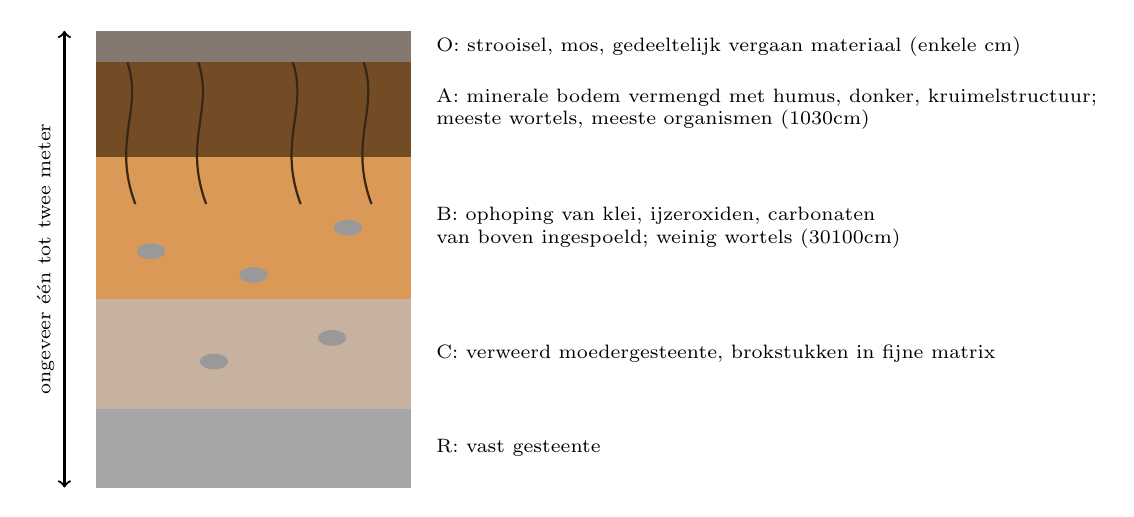
\begin{tikzpicture}[every node/.style={font=\scriptsize}]
  \fill[brown!25!black!60] (0,5.4) rectangle (4,5.8); \node[right] at (4.2,5.6) {O: strooisel, mos, gedeeltelijk vergaan materiaal (enkele cm)};
  \fill[brown!60!black] (0,4.2) rectangle (4,5.4); \node[right, align=left] at (4.2,4.8) {A: minerale bodem vermengd met humus, donker, kruimelstructuur;\\ meeste wortels, meeste organismen (\qtyrange{10}{30}{cm})};
  \fill[brown!70!orange!80] (0,2.4) rectangle (4,4.2); \node[right, align=left] at (4.2,3.3) {B: ophoping van klei, ijzeroxiden, carbonaten\\ van boven ingespoeld; weinig wortels (\qtyrange{30}{100}{cm})};
  \fill[gray!50!brown!60] (0,1.0) rectangle (4,2.4); \node[right, align=left] at (4.2,1.7) {C: verweerd moedergesteente, brokstukken in fijne matrix};
  \fill[gray!70] (0,0) rectangle (4,1.0); \node[right] at (4.2,0.5) {R: vast gesteente};
  \foreach \x in {0.4,1.3,2.5,3.4} \draw[brown!30!black, thick] (\x,5.4) .. controls (\x+0.2,4.8) and (\x-0.2,4.4) .. (\x+0.1,3.6);
  \foreach \x/\y in {0.7/3.0, 2.0/2.7, 3.2/3.3, 1.5/1.6, 3.0/1.9} \fill[gray!80] (\x,\y) ellipse (0.18 and 0.1);
  \draw[<->, thick] (-0.4,5.8) -- (-0.4,0) node[midway, left, rotate=90, anchor=south] {ongeveer één tot twee meter};
\end{tikzpicture}

{\small Een bodemprofiel. Organisch materiaal komt bovenaan binnen en wordt
verbruikt terwijl het afdaalt; mineraal materiaal komt onderaan vrij en wordt
door wortels en dieren naar boven verplaatst; opgeloste stoffen reizen met het
water naar beneden en worden in de B-horizont opgevangen.}
\end{omfigure}

\begin{proposition}[Waarom klei en humus ertoe doen]\label{prop:b2:living-soil:cec}
\index{kationuitwisselingscapaciteit}\index{klei}\index{bodemstructuur}\index{veldcapaciteit}
Kleideeltjes en \omterm{def:b2:living-soil:soil}{humus} dragen negatieve ladingen aan hun oppervlak en houden
door elektrostatische aantrekking een voorraad uitwisselbare kationen vast
--- $\mathrm{Ca^{2+}}$, $\mathrm{Mg^{2+}}$, $\mathrm{K^{+}}$, $\mathrm{NH_4^{+}}$ --- waaruit
plantenwortels putten door er $\mathrm{H^{+}}$ tegen uit te wisselen. Deze
\emph{\omterm{prop:b2:living-soil:cec}{kationuitwisselingscapaciteit}} is de voedingsbank van de \omterm{def:b2:living-soil:soil}{bodem}; een
zandgrond heeft er bijna geen (enkele centimol lading per kilogram), een
humusrijke kleiige leem vijftig keer meer, en de vruchtbaarheid van beide
verschilt navenant. Dezelfde oppervlakken houden water vast: een zandgrond
draineert binnen een dag tot een \emph{\omterm{prop:b2:living-soil:cec}{veldcapaciteit}} van een tiende van zijn
volume, een leem houdt een derde vast, en het verschil is wat een gewas tussen
twee regenbuien heeft. En \omterm{def:b2:living-soil:soil}{humus} plakt, samen met schimmeldraden,
wortelexsudaten en het slijm van wormen, minerale korrels aaneen tot
\emph{aggregaten}, de kruimelstructuur waarvan de poriën lucht, water en
wortels doorlaten --- de eigenschap die een \omterm{def:b2:living-soil:soil}{bodem} van een sediment
onderscheidt en die als eerste wordt vernietigd door ploegen en verdichting.
\end{proposition}

\section{Wie er leeft}

\begin{proposition}[De bodemgemeenschap]\label{prop:b2:living-soil:community}
\index{bodemvoedselweb}\index{detritivoor}\index{regenworm}\index{bodembiomassa}
Een gram vruchtbare bovengrond bevat ongeveer $10^{9}$ bacteriecellen van
zo'n tienduizend soorten, honderd meter schimmeldraden, $10^{4}$
\omterm{def:b2:unicellular-diversity:protist}{protisten}, enkele tientallen nematoden en een handvol mijten en
springstaarten; een vierkante meter bevat enkele honderden regenwormen en,
onder de zichtbare dieren, een levende massa van meerdere ton per
hectare --- vergelijkbaar met het vee dat dezelfde hectare zou kunnen dragen.
De gemeenschap is een \emph{detritusvoedselweb}: bacteriën en schimmels
(de \emph{afbrekers}) eten dood materiaal en worden gegeten door \omterm{def:b2:unicellular-diversity:protist}{protisten}
en nematoden (de microbiële grazers), die worden gegeten door mijten en
roofnematoden, die op hun beurt duizendpoten en kevers voeden; de
\emph{detritivoren} --- regenwormen, miljoenpoten, pissebedden, termieten,
springstaarten --- eten het strooisel zelf met de microben erop, en
versnipperen het duizendvoudig, zodat het oppervlak dat de microben aanvallen
vermenigvuldigt. De grazers doen ertoe boven hun aantallen uit: door bacteriën
te eten, maken ze de stikstof die in bacteriecellen vastzit vrij als
ammonium, en een \omterm{def:b2:living-soil:soil}{bodem} met \omterm{def:b2:unicellular-diversity:protist}{protisten} en nematoden mineraliseert
stikstof sneller dan een \omterm{def:b2:living-soil:soil}{bodem} met alleen bacteriën. Regenwormen zijn de
\emph{ecosysteemingenieurs}: hun gangen zijn de macroporiën van de \omterm{def:b2:living-soil:soil}{bodem}, hun
uitwerpselen de rijkste aggregaten, en de wormen van een grasland voeren elk
jaar enkele ton aarde per hectare door hun darmen, zoals Darwin mat.
\end{proposition}

\begin{omfigure}
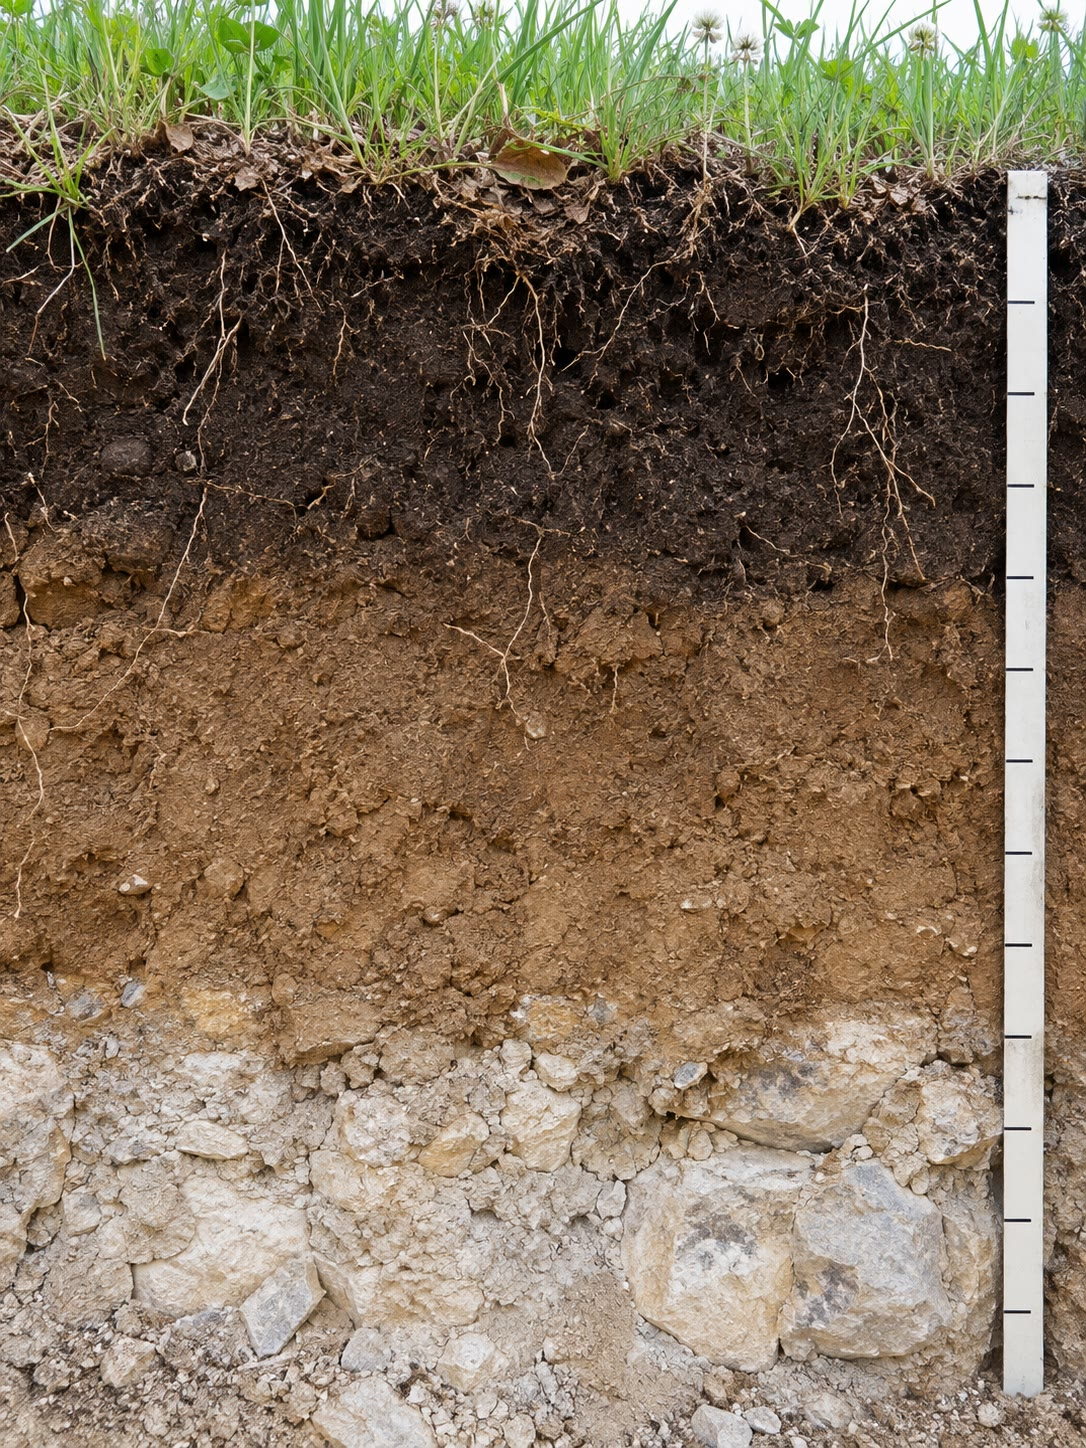
\includegraphics[width=0.21\linewidth]{images/book4/ai/b4-26-soil-profile.jpg}\hspace{0.025\linewidth}
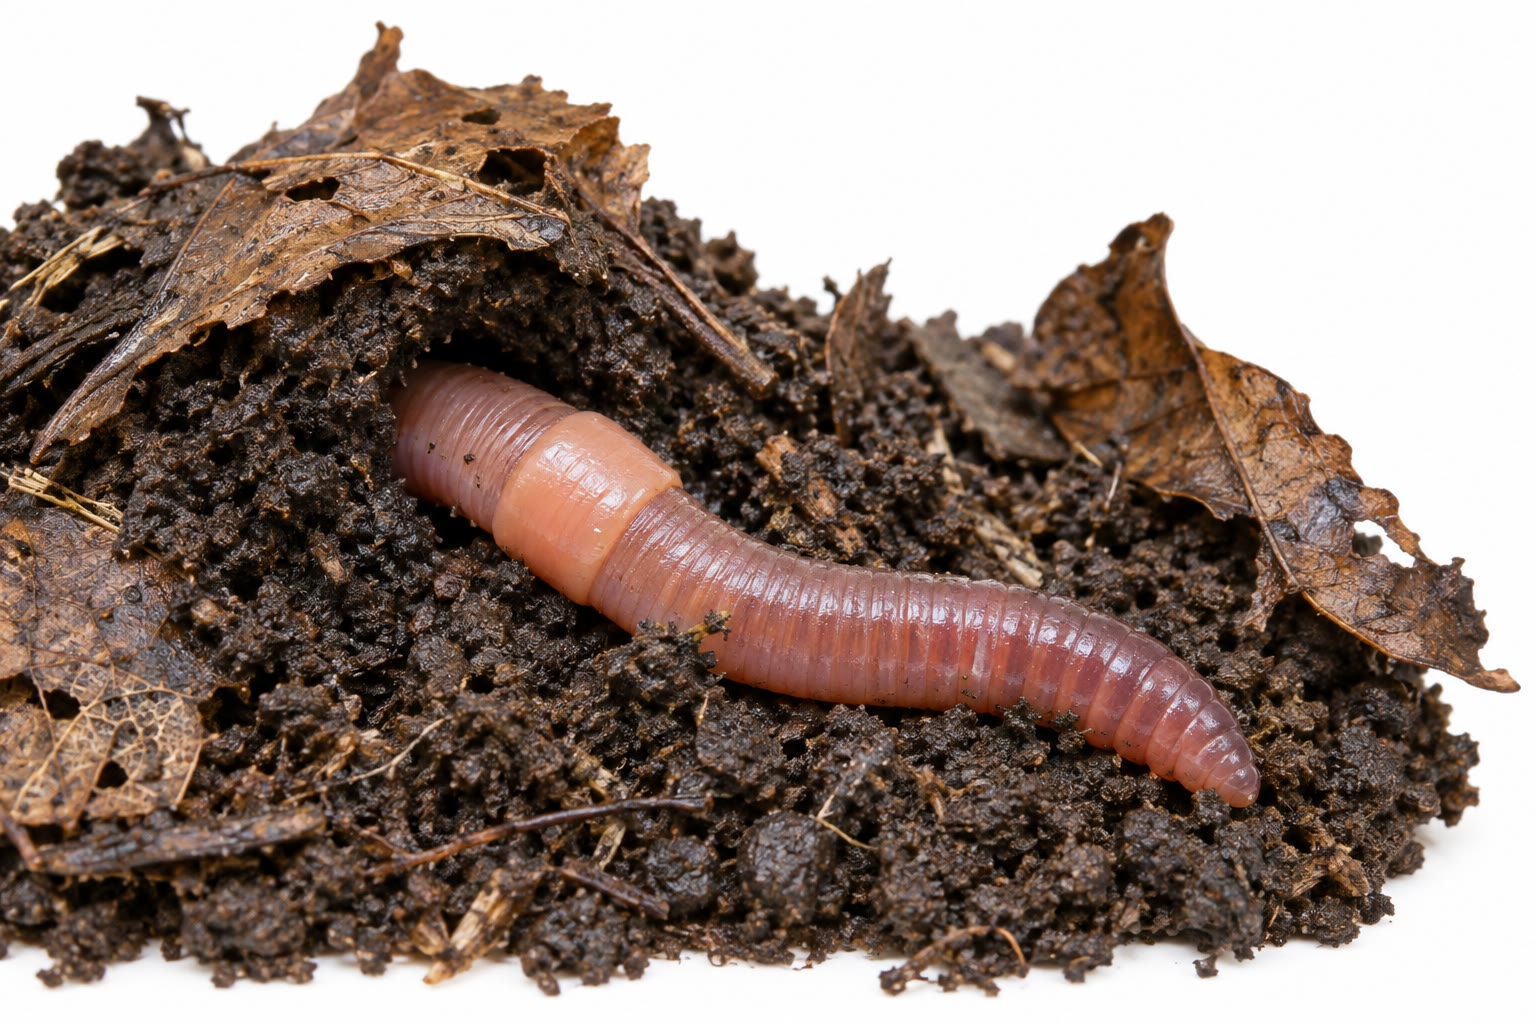
\includegraphics[width=0.42\linewidth]{images/book4/ai/b4-26-earthworm.jpg}\hspace{0.025\linewidth}
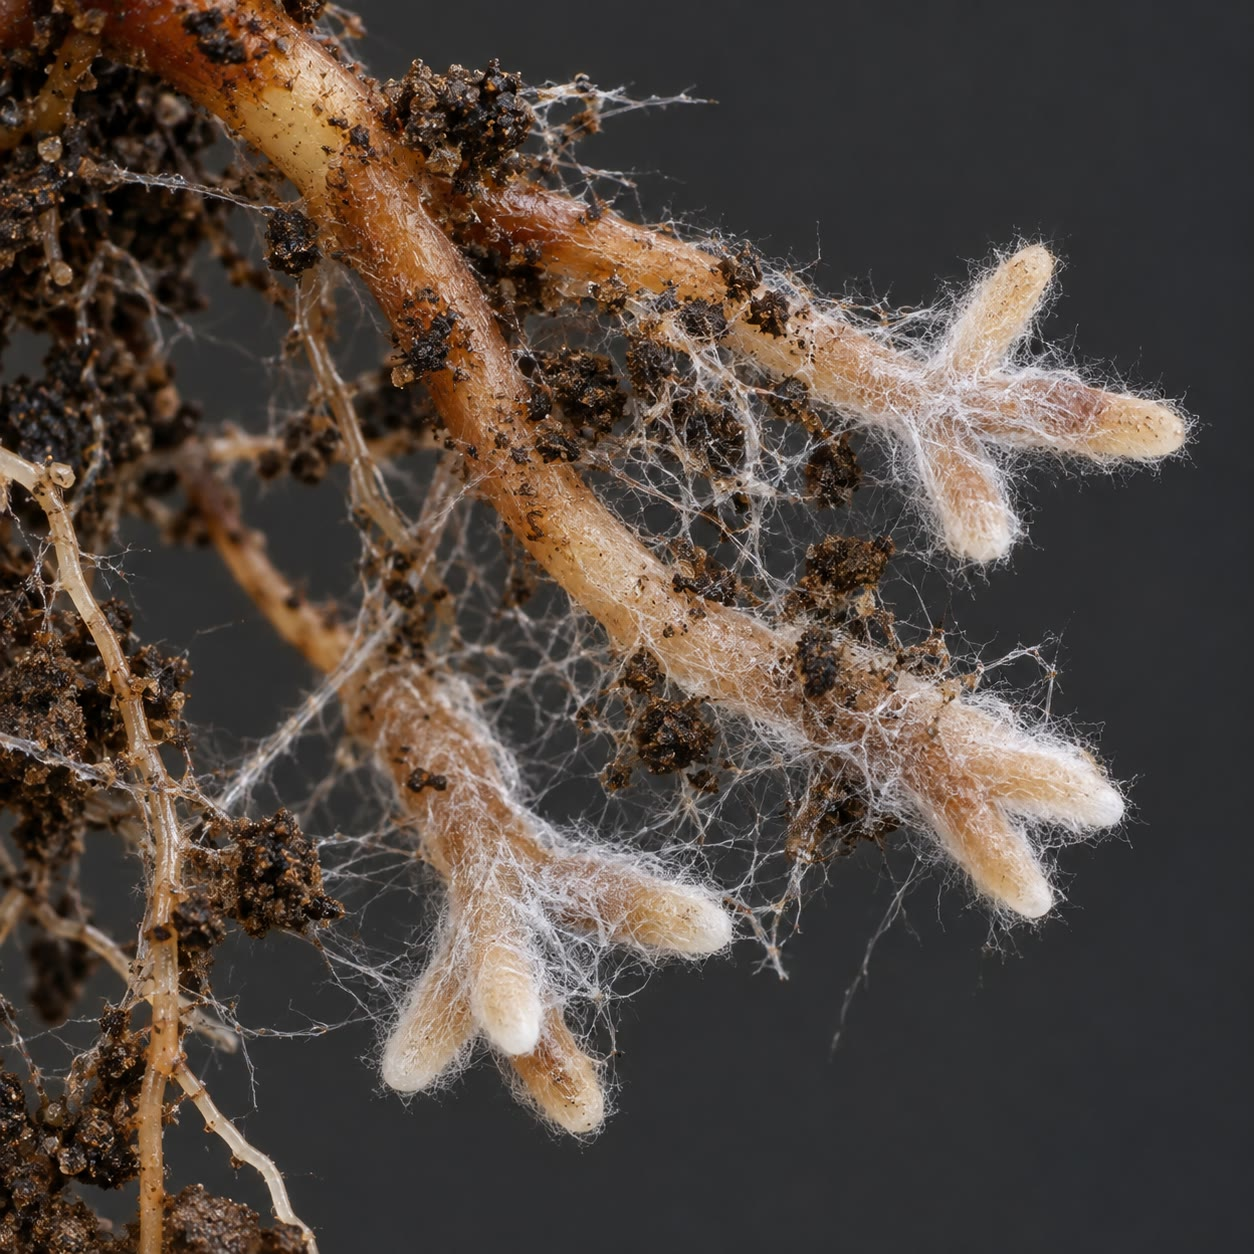
\includegraphics[width=0.28\linewidth]{images/book4/ai/b4-26-mycorrhiza.jpg}

{\small De \omterm{def:b2:living-soil:soil}{bodem} en twee van zijn makers. Links: een profiel in een
afgegraven talud, donkere bovengrond die naar beneden overgaat in bleek
verweerd gesteente. Midden: een regenworm in zijn gang. Rechts: een wortel met
zijn ectomycorrhizamantel en de schimmeldraden die hem in de \omterm{def:b2:living-soil:soil}{bodem} verlengen.}
\end{omfigure}

\section{Afbraak}

\begin{theorem}[Strooiselafbraak en de verhouding tussen koolstof en stikstof]\label{thm:b2:living-soil:decay}
\index{afbraak}\index{strooiselafbraak}\index{C:N-verhouding}\index{mineralisatie}\index{immobilisatie}
Strooisel breekt af met een snelheid evenredig met wat er nog is,
$\mathrm{d}L/\mathrm{d}t = -kL$, dus $L = L_0 e^{-kt}$ met een
\emph{afbraakconstante} $k$ van ongeveer 1 per jaar voor gras en
bladeren van loofbomen in een gematigd bos, $0.3$ voor naalden van coniferen,
meerdere per jaar in de natte tropen en $0.05$ in de toendra;
een constante aanvoer $I$ per jaar bouwt een strooisellaag van $I/k$ op. De
afbraak wordt bepaald door temperatuur, vocht en de \emph{kwaliteit} van het
strooisel: stikstofgehalte, ligninegehalte en de verhouding tussen koolstof en
stikstof. Microben hebben $\mathrm{C:N} \approx 8$ en
houden ongeveer \qty{40}{\%} vast van de koolstof die ze eten, zodat ze één
stikstof nodig hebben voor elke $8/0.4 = 20$ koolstofatomen voedsel: strooisel
met $\mathrm{C:N}$ onder ongeveer 25 maakt bij de afbraak ammonium vrij
(\emph{mineralisatie}), terwijl strooisel daarboven --- stro met 80,
\omterm{def:b2:plant-meristems:wood}{hout} met 400 --- de microben stikstof uit de \omterm{def:b2:living-soil:soil}{bodem} laat opnemen
(\emph{immobilisatie}), waardoor de planten tekortkomen tot de koolstof is
weggeademd en de verhouding is gedaald. Daarom drukt vers ondergeploegd stro
een gewas, voedt het residu van vlinderbloemigen het, en heeft een composthoop
beide nodig.
\end{theorem}
\begin{proof}
Voor de verhouding: microben die strooisel met $c$ koolstofatomen per
stikstof eten, assimileren $0.4c$ koolstofatomen en hebben, om biomassa op te
bouwen met $\mathrm{C:N} = 8$, $0.4c/8 = c/20$ stikstofatomen nodig; het
strooisel levert er 1. Als $c < 20$ is er stikstof over, die als ammonium
vrijkomt; als $c > 20$ is er een tekort dat uit de \omterm{def:b2:living-soil:soil}{bodem} wordt gehaald. De
drempel 25 in de praktijk weerspiegelt een retentie-efficiëntie iets
onder 0.4. Voor de strooisellaag: $\mathrm{d}L/\mathrm{d}t = I - kL$
heeft als \omterm{def:b2:biogeochemical-cycles:reservoir}{stationaire toestand} $I/k$, bereikt met tijdconstante $1/k$; de
\omterm{def:b2:biogeochemical-cycles:reservoir}{verblijftijd} van strooisel is $1/k$, één jaar in een beukenbos en
twintig in de toendra.
\end{proof}
\begin{proof}[Bewijsmateriaal]
Strooiselzakexperimenten --- bekende massa's bladeren in gaaszakjes,
begraven en met tussenpozen gewogen --- leverden de exponentiële wet en haar
constanten in elk bioom op (Olson, 1963), en toonden met verschillende
maaswijdtes aan dat het uitsluiten van de bodemdieren de snelheid halveert:
de microben doen de chemie, maar de dieren bepalen het tempo. Over een heel
continent breekt hetzelfde blad in Georgia in een jaar af en in Alaska in
acht, in verhouding tot de werkelijke evapotranspiratie, het product van
warmte en water.
\end{proof}

\begin{omfigure}
\begin{tikzpicture}
\begin{axis}[
  width=0.72\linewidth, height=5.6cm,
  axis x line=bottom, axis y line=left,
  xmin=0, xmax=6, ymin=0, ymax=105,
  xlabel={jaren}, ylabel={resterende strooiselmassa (\%)},
  xlabel style={font=\small, at={(axis description cs:0.5,-0.13)}, anchor=north},
  ylabel style={font=\small},
  tick label style={font=\small},
  legend style={font=\scriptsize, at={(0.5,-0.3)}, anchor=north, draw=none, legend columns=2},
  clip=false,
]
\addplot[very thick, omDef, domain=0:6, samples=60] {100*exp(-2*x)};
\addlegendentry{blad uit tropisch bos, $k = 2$}
\addplot[very thick, omThm, domain=0:6, samples=60] {100*exp(-1*x)};
\addlegendentry{beukenblad, $k = 1$}
\addplot[very thick, omProp, domain=0:6, samples=60] {100*exp(-0.3*x)};
\addlegendentry{sparrennaald, $k = 0.3$}
\addplot[very thick, gray, domain=0:6, samples=60] {100*exp(-0.05*x)};
\addlegendentry{toendramos, $k = 0.05$}
\end{axis}
\end{tikzpicture}

{\small Exponentiële afbraak van strooisel. De helft van een beukenblad is na
acht maanden verdwenen, de helft van een toendramos na veertien jaar; het
residu dat microben noch dieren kunnen afmaken, wordt \omterm{def:b2:living-soil:soil}{humus}.}
\end{omfigure}

\begin{proposition}[Humus en de koolstofvoorraad van de bodem]\label{prop:b2:living-soil:humus}
\index{humus}\index{organische bodemkoolstof}\index{bodemademhaling}
Enkele procenten van de koolstof van het strooisel ontsnappen aan volledige
oxidatie en worden \emph{\omterm{def:b2:living-soil:soil}{humus}}: een donker, amorf mengsel van microbiële
resten, veranderd lignine en plantaardige verbindingen, gebonden aan klei en
ijzer en opgesloten in aggregaten, dat afbreekt met \omterm{def:b2:biogeochemical-cycles:reservoir}{verblijftijden} van
decennia tot millennia. In \omterm{def:b2:living-soil:soil}{humus} zetelt de vruchtbaarheid van de \omterm{def:b2:living-soil:soil}{bodem}
--- het grootste deel van zijn stikstof en kationuitwisseling, de helft van zijn
watervasthoudend vermogen --- en \omterm{def:b2:living-soil:soil}{humus} is de grootste voorraad organische
koolstof op land, \qty{1700}{GtC} in de bovenste meter, twee keer die van de
atmosfeer. Zijn balans is aanvoer min afbraak, $\mathrm{d}H/\mathrm{d}t = I_h - k_hH$:
met $k_h \approx 0.02$ per jaar bevat een \omterm{def:b2:living-soil:soil}{bodem} vijftig jaar aanvoer,
en elke verandering --- ploegen, dat de aggregaten breekt en de \omterm{def:b2:living-soil:soil}{humus} belucht;
het draineren van een veen, dat zuurstof binnenlaat; opwarming, die $k_h$
verhoogt --- toont zich als een verlies dat decennia aanhoudt. De
landbouwbodems van de wereld hebben sinds ze voor het eerst werden omgeploegd
een derde tot de helft van hun \omterm{def:b2:living-soil:soil}{humus} verloren, zo'n
\qty{100}{GtC}, en een opwarming van \qty{3}{\celsius} zou de afbraak van de
rest met een derde verhogen: \omterm{def:b2:living-soil:soil}{bodems} zijn de grootste onzekerheid in het
koolstofbudget van \cref{ch:b2:global-change}.
\end{proposition}

\section{Partnerschappen onder de grond}

\begin{proposition}[Mycorrhiza's en rhizobia]\label{prop:b2:living-soil:symbiosis}
\index{mycorrhiza}\index{rhizobium}\index{wortelknolletje}\index{nitrogenase}\index{leghemoglobine}
Bij negen op de tien plantensoorten worden de wortels door schimmels
gekoloniseerd in een \emph{mycorrhiza}: de plant geeft suiker (een tiende tot
een vijfde van haar fotosyntheseproducten) en de schimmel geeft fosfaat,
stikstof, water en zink, die zijn schimmeldraden, honderd keer dunner dan een
wortel en per eenheid koolstof honderd keer zo lang, verzamelen uit een
bodemvolume dat de wortel niet kan bereiken --- vooral fosfaat, dat zo traag
door de \omterm{def:b2:living-soil:soil}{bodem} diffundeert dat een wortel zijn millimeter omgeving binnen enkele
dagen uitput. \emph{Arbusculaire} mycorrhiza's, de oudste soort, dringen de
wortelcellen binnen en vertakken zich tot arbuscules waar de uitwisseling
plaatsvindt; de \emph{ectomycorrhiza's} van bosbomen omhullen de wortelpunt en
groeien tussen de cellen ervan. Vlinderbloemigen gaan verder: rhizobia, die
door de flavonoïden van de wortel worden aangetrokken, dringen binnen via een
wortelhaar, en de wortel bouwt er een \emph{wortelknolletje} omheen waarin de
bacteriën, als \emph{bacteroïden}, stikstof binden met nitrogenase --- een
enzym dat zo gevoelig is voor zuurstof dat het knolletje bijna anoxisch moet
worden gehouden door \emph{leghemoglobine}, een hemoglobine die de plant maakt,
die het knolletje zijn roze kleur geeft en zuurstof aan de bacteroïden levert
in een concentratie die te laag is om het enzym te vergiftigen. Elke partner
controleert de andere: een plant snijdt de suiker af voor knolletjes die niets
binden, en een schimmel die minder fosfaat levert, krijgt minder
koolstof.
\end{proposition}
\begin{proof}[Bewijsmateriaal]
Kiers en collega's (2011) kweekten een plant met twee schimmelpartners op
een gesplitst wortelstelsel en boden aan één kant fosfaat aan:
de plant wees meer koolstof toe aan de schimmel die meer fosfaat leverde, en de
schimmel wees meer fosfaat toe aan een wortel die meer koolstof gaf ---
wederzijdse beloningen, gemeten met isotopen. Bij rhizobia kregen knolletjes
die experimenteel geen stikstof konden binden (door de lucht te vervangen door
argon en zuurstof) minder zuurstof en groeiden ze minder dan knolletjes op
dezelfde plant die wel konden binden: de plant bestraft valsspelers.
Stikstof-15-tracering toont aan dat een grasmat van klaver en gras binnen één
seizoen een derde van de door klaver gebonden stikstof aan het gras
overdraagt, via de \omterm{def:b2:living-soil:soil}{bodem} en via gedeelde schimmelnetwerken.
\end{proof}

\begin{omfigure}
\begin{tikzpicture}[every node/.style={font=\scriptsize}, >=stealth]
  % root cross-section
  \fill[omThm!15] (0,0) circle (1.5); \draw[thick] (0,0) circle (1.5);
  \fill[omThm!30] (0,0) circle (0.5); \draw[thick] (0,0) circle (0.5);
  \node at (0,0) {centrale cilinder};
  \node at (0,1.05) {schors};
  % arbuscules in cortex cells
  \foreach \a in {30,150,270} { \draw[omDef, thick] ({1.0*cos(\a)},{1.0*sin(\a)}) -- ++({0.25*cos(\a+60)},{0.25*sin(\a+60)}) -- ++({0.2*cos(\a-40)},{0.2*sin(\a-40)}); \draw[omDef, thick] ({1.0*cos(\a)},{1.0*sin(\a)}) -- ++({0.25*cos(\a-60)},{0.25*sin(\a-60)}); }
  % hyphae out
  \foreach \a in {20,80,150,210,340} { \draw[omDef, thick] ({1.5*cos(\a)},{1.5*sin(\a)}) .. controls ({2.2*cos(\a+10)},{2.2*sin(\a+10)}) .. ({2.7*cos(\a-5)},{2.7*sin(\a-5)}); }
  \draw[omDef, thick] ({1.5*cos(150)},{1.5*sin(150)}) -- ({1.0*cos(150)},{1.0*sin(150)});
  \node[omDef, anchor=west, align=left] at (2.9,1.4) {schimmeldraden: \qty{3}{\micro m} breed,\\ meters per centimeter wortel};
  \node[omDef, anchor=west] at (2.9,0.1) {arbuscule in een schorscel};
  \draw[omDef] (2.85,0.1) -- (1.2,0.5);
  \node[anchor=north, align=center] at (0,-1.6) {wortel, \qty{0.3}{mm} doorsnede};
  \draw[->, thick, omThm] (-1.2,-2.4) -- (1.2,-2.4) node[right] {suiker naar de schimmel, \qtyrange{10}{20}{\%} van de fotosyntheseproducten};
  \draw[<-, thick, omDef] (-1.2,-2.9) -- (1.2,-2.9) node[right] {fosfaat, ammonium, water, zink naar de plant};
  % nodule
  \begin{scope}[xshift=9.3cm]
    \draw[thick, brown!60!black] (-0.3,2.4) -- (-0.1,-0.6);
    \draw[thick, brown!60!black] (-0.1,0.3) -- (1.6,0.1);
    \fill[pink!60!red!40] (1.5,0.2) circle (0.9); \draw[thick] (1.5,0.2) circle (0.9);
    \fill[pink!80!red!60] (1.5,0.2) circle (0.55);
    \foreach \p in {(1.3,0.3),(1.6,0.0),(1.5,0.45),(1.7,0.3),(1.35,0.05)} \fill[omDef!70!black] \p ellipse (0.08 and 0.05);
    \node[anchor=north, align=center] at (1.5,-0.8) {knolletje: bacteroïden in plantencellen,\\ roze door leghemoglobine;\\ zuurstof op \qty{10}{nM}, zodat nitrogenase\\ werkt en de cellen toch ademen};
    \node[anchor=south, align=center] at (-0.2,2.45) {wortel van een vlinderbloemige};
  \end{scope}
\end{tikzpicture}

{\small Twee afspraken. Links: een arbusculaire mycorrhiza, suiker naar buiten
en fosfaat naar binnen via arbuscules in de schorscellen. Rechts:
een wortelknolletje van een vlinderbloemige, waar de eigen hemoglobine van de
plant de zuurstof laag genoeg houdt voor nitrogenase en hoog genoeg voor de
ademhaling.}
\end{omfigure}

\section{Bodem verliezen}

\begin{proposition}[Erosie, zout en de balans van een bodem]\label{prop:b2:living-soil:erosion}
\index{bodemerosie}\index{verzilting}\index{woestijnvorming}
\omterm{def:b2:living-soil:soil}{Bodem} vormt zich met \qtyrange{0.05}{0.5}{mm} per jaar en erodeert onder
natuurlijke vegetatie ongeveer even snel. Kaal geploegd land op een
helling verliest \qtyrange{1}{10}{mm} per jaar aan water en wind ---
\qtyrange{10}{100}{t/ha} --- tien tot honderd keer het tempo van de
vorming: een \omterm{def:b2:living-soil:soil}{bodem} die in tienduizend jaar is opgebouwd, is in een eeuw
verdwenen, en daarmee de \omterm{def:b2:living-soil:soil}{humus} en de voedingsstoffen van de A-horizont,
het enige deel dat ertoe doet. Groenbemesters, terrassen, ploegen volgens de
hoogtelijnen en niet-kerende landbouw, die het residu aan het oppervlak laat en
de aggregaten intact houdt, brengen het verlies terug tot bij het tempo van de
vorming. Irrigatie in droge klimaten brengt het tegenovergestelde falen:
water verdampt en laat zijn zouten achter, een ton per hectare per jaar uit
water dat maar licht zout is, tot de osmotische potentiaal van de
bodemoplossing (\cref{ch:b2:plant-plasticity}) lager is dan de wortels kunnen
overwinnen --- \emph{verzilting}, die vierduizend jaar geleden de akkers van
Sumer buiten gebruik stelde en nu een vijfde van het geïrrigeerde land treft.
De toestand van een \omterm{def:b2:living-soil:soil}{bodem} is een budget: \omterm{def:b2:living-soil:soil}{humus} erin tegenover \omterm{def:b2:living-soil:soil}{humus} eruit,
vorming tegenover erosie, zout erin tegenover zout afgevoerd; elk heeft een
\omterm{def:b2:biogeochemical-cycles:reservoir}{verblijftijd}, en elk is, eenmaal negatief, traag om te keren.
\end{proposition}

\section{Opgaven}

\begin{exercise}[$\star$]\label{exo:b2:living-soil:1}
Noem de horizonten van een bodemprofiel van het oppervlak naar beneden en zeg
wat er in elk gebeurt.
\end{exercise}

\begin{exercise}[$\star$]\label{exo:b2:living-soil:2}
Leg uit wat \omterm{prop:b2:living-soil:cec}{kationuitwisselingscapaciteit} is, waarom een zandgrond er weinig
van heeft, en wat een boer doet die een zure \omterm{def:b2:living-soil:soil}{bodem} bekalkt.
\end{exercise}

\begin{exercise}[$\star$]\label{exo:b2:living-soil:3}
Noem de belangrijkste groepen van het \omterm{prop:b2:living-soil:community}{bodemvoedselweb}, van afbrekers tot
toppredatoren, met telkens één organisme, en zeg wat de grazers van
bacteriën voor de planten doen.
\end{exercise}

\begin{exercise}[$\star$]\label{exo:b2:living-soil:4}
Onderscheid arbusculaire mycorrhiza's en ectomycorrhiza's, en zeg wat elke
partner geeft en krijgt.
\end{exercise}

\begin{exercise}[$\star\star$]\label{exo:b2:living-soil:5}
Een beukenbos laat per jaar \qty{4}{t/ha} bladeren vallen, en de
\omterm{thm:b2:living-soil:decay}{strooiselafbraak} verloopt met $k = 0.8$ per jaar. Bereken de strooiselmassa in \omterm{def:b2:biogeochemical-cycles:reservoir}{stationaire
toestand}, de \omterm{def:b2:biogeochemical-cycles:reservoir}{verblijftijd} van het strooisel, en de tijd waarin de bladval van
één jaar \qty{90}{\%} van zijn massa verliest.
\end{exercise}

\begin{exercise}[$\star\star$]\label{exo:b2:living-soil:6}
Tarwestro heeft $\mathrm{C:N} = 80$ en klaverresidu $15$. Bereken voor
elk de stikstof die de microben nodig hebben per \qty{100}{kg}
verbruikte koolstof (retentie 0.4, microbiële $\mathrm{C:N} = 8$) en
of het residu mineraliseert of immobiliseert, en hoeveel.
\end{exercise}

\begin{exercise}[$\star\star$]\label{exo:b2:living-soil:7}
Een hectare grasland bevat \qty{2}{t} regenwormen die elk per jaar tien keer
hun massa aan aarde verwerken. Bereken de aarde die per jaar door wormen gaat
en de tijd waarin de bovenste \qty{20}{cm} (volumieke massa
\qty{1.3}{t/m^3}) er één keer doorheen is gegaan. Vergelijk met het getal van
Darwin.
\end{exercise}

\begin{exercise}[$\star\star$]\label{exo:b2:living-soil:8}
Een gram \omterm{def:b2:living-soil:soil}{bodem} bevat $10^{9}$ bacteriën van elk \qty{e-12}{g},
en \qty{100}{m} schimmeldraden met een diameter van \qty{4}{\micro m} en een
dichtheid van \qty{1.1}{g/cm^3}. Bereken de bacteriële en schimmelbiomassa per
gram en per hectare (bovenste \qty{20}{cm}, \qty{1.3}{t/m^3}).
\end{exercise}

\begin{exercise}[$\star\star$]\label{exo:b2:living-soil:9}
Bodemhumus breekt af met $k_h = 0.02$ per jaar en ontvangt
\qty{1.5}{t/ha} koolstof per jaar. Bereken de humuskoolstof in \omterm{def:b2:biogeochemical-cycles:reservoir}{stationaire
toestand}. Het veld wordt geploegd en $k_h$ verdubbelt: bereken de nieuwe
\omterm{def:b2:biogeochemical-cycles:reservoir}{stationaire toestand}, de verloren koolstof, en de tijd waarin de helft ervan
verloren gaat.
\end{exercise}

\begin{exercise}[$\star\star\star$]\label{exo:b2:living-soil:10}
Fosfaat diffundeert door de \omterm{def:b2:living-soil:soil}{bodem} met $D \approx \qty{e-13}{m^2/s}$.
Bereken hoe ver het in een groeiseizoen van \num{100} dagen komt
($x \approx \sqrt{2Dt}$), en vergelijk met de afstand tussen wortels
(\qty{1}{cm}) en tussen schimmeldraden (\qty{0.1}{mm}). Wat zegt dit
over waarom mycorrhiza's belangrijk zijn voor fosfor en minder voor nitraat
($D \approx \qty{e-10}{m^2/s}$)?
\end{exercise}

\begin{exercise}[$\star\star\star$]\label{exo:b2:living-soil:11}
Een helling verliest per jaar \qty{20}{t/ha} \omterm{def:b2:living-soil:soil}{bodem} door erosie en
vormt er \qty{1}{t/ha}; de A-horizont is \qty{25}{cm} dik, heeft
\qty{1.3}{t/m^3} en bevat \qty{3}{\%} koolstof. Bereken de massa van de
A-horizont, zijn levensduur in dit tempo, en de koolstof die per jaar
verloren gaat. Bij niet-kerende landbouw daalt het verlies tot \qty{2}{t/ha}:
bereken de levensduur opnieuw.
\end{exercise}

\begin{exercise}[$\star\star\star$]\label{exo:b2:living-soil:12}
``De \omterm{def:b2:living-soil:soil}{bodem} is het traagste organisme op de boerderij.'' Bespreek dit met de
\omterm{def:b2:biogeochemical-cycles:reservoir}{verblijftijden} van strooisel, \omterm{def:b2:living-soil:soil}{humus}, minerale \omterm{def:b2:living-soil:soil}{bodem} en zout, en zeg
welke veranderingen een boer binnen een loopbaan kan zien en welke niet.
\end{exercise}

\section{Vraagstuk: een hectare bodem}

\begin{problem}[{Weekendvraagstuk --- een hectare akkerbodem
doorgelicht: de levende massa geteld, het strooisel en de humus gevolgd
door hun exponentiële budgetten, de stikstof die een residu van
vlinderbloemigen vrijmaakt afgezet tegen de behoefte van een gewas, en de
erosie- en koolstofrekeningen van twee beheersvormen vergeleken, met als
besluit de koolstofvoorraad van de bodem, zijn levensduur onder de ploeg en de
stikstof die een vlinderbloemige levert}]
\label{pb:b2:living-soil:1}
De hectare: A-horizont \qty{25}{cm} dik, volumieke massa
\qty{1.3}{t/m^3}, \qty{2.5}{\%} organische koolstof; humusafbraak $k_h =
0.025$ per jaar onder de ploeg, $0.015$ bij niet-kerende landbouw; koolstofaanvoer
naar de \omterm{def:b2:living-soil:soil}{humus} in beide gevallen \qty{1.2}{t/ha} per jaar. Strooisel: een
klaver als groenbemester laat \qty{5}{t/ha} droge stof achter met
\qty{45}{\%} koolstof en \qty{3}{\%} stikstof, die afbreekt met $k = 2$
per jaar. Erosie: \qty{15}{t/ha} per jaar bij ploegen, \qty{1.5}{t/ha}
bij niet-kerende landbouw; vorming \qty{0.5}{t/ha}.

\medskip
\noindent\textbf{Deel I --- De voorraad.}
\begin{enumerate}
  \item Bereken de massa van de A-horizont en zijn organische koolstof.
  \item Bereken de massa stikstof in de \omterm{def:b2:living-soil:soil}{humus} als de
        $\mathrm{C:N}$ ervan 12 is.
  \item De \omterm{def:b2:living-soil:soil}{bodem} bevat $10^{9}$ bacteriën per gram van elk \qty{e-12}{g}
        en \qty{200}{m} schimmeldraden per gram met een diameter van
        \qty{4}{\micro m}, dichtheid 1.1. Bereken de microbiële biomassa per
        hectare.
  \item Tel er \qty{1.5}{t/ha} regenwormen en \qty{0.2}{t/ha}
        andere dieren bij, en geef de totale levende massa per hectare.
        Welke fractie van de humuskoolstof is dat?
  \item De microben vernieuwen hun biomassa twee keer per jaar en ademen
        \qty{60}{\%} van wat ze eten. Schat de koolstof die ze per jaar
        verbruiken, en het geademde $\mathrm{CO_2}$.
  \item Vergelijk met de netto primaire productie van het gewas van ongeveer
        \qty{5}{t/ha} koolstof en geef commentaar.
\end{enumerate}

\medskip
\noindent\textbf{Deel II --- Het klaverresidu.}
\begin{enumerate}[resume]
  \item Bereken de koolstof en de stikstof in het residu en de
        $\mathrm{C:N}$ ervan.
  \item Mineraliseert of immobiliseert het residu stikstof, met microbiële
        $\mathrm{C:N} = 8$ en retentie $0.4$? Bereken de netto vrijgemaakte
        stikstof wanneer het hele residu afbreekt.
  \item Welke fractie van het residu is met $k = 2$ na 3 maanden afgebroken?
        Na een jaar?
  \item Bereken de stikstof die in de eerste 3 maanden vrijkomt.
  \item Een tarwegewas neemt \qty{150}{kg} stikstof per hectare op,
        grotendeels in de twee maanden na het zaaien. Geef commentaar op de
        timing.
  \item In plaats daarvan wordt dezelfde massa tarwestro ($\mathrm{C:N} = 80$)
        ondergeploegd. Bereken de geïmmobiliseerde stikstof en
        zeg wat de boer moet doen.
\end{enumerate}

\medskip
\noindent\textbf{Deel III --- \omterm{def:b2:living-soil:soil}{Humus}.}
\begin{enumerate}[resume]
  \item Bereken de humuskoolstof in \omterm{def:b2:biogeochemical-cycles:reservoir}{stationaire toestand} onder de ploeg en
        bij niet-kerende landbouw.
  \item Het veld, in de \omterm{def:b2:biogeochemical-cycles:reservoir}{stationaire toestand} onder de ploeg, wordt omgezet naar
        niet-kerende landbouw. Schrijf $H(t)$ op en bereken de gewonnen koolstof
        na 10 en 50 jaar.
  \item Bereken het tempo van de winst in het eerste jaar, in ton
        koolstof per hectare, en in ton $\mathrm{CO_2}$.
  \item Als de \qty{1.5e9}{ha} akkerland van de wereld hetzelfde deed,
        hoe groot zou de put in het eerste jaar dan zijn, tegenover een fossiele
        uitstoot van \qty{10}{GtC}? En in het vijftigste jaar?
  \item Waarom is de put tijdelijk en omkeerbaar?
  \item Een opwarming van \qty{3}{\celsius} verhoogt $k_h$ met een derde.
        Bereken de nieuwe \omterm{def:b2:biogeochemical-cycles:reservoir}{stationaire toestand} bij niet-kerende landbouw en de
        verloren koolstof.
\end{enumerate}

\medskip
\noindent\textbf{Deel IV --- Erosie.}
\begin{enumerate}[resume]
  \item Bereken het netto bodemverlies per jaar in elk beheer.
  \item Bereken de levensduur van de A-horizont in elk beheer.
  \item Bereken de koolstof en stikstof die onder de ploeg per jaar door
        erosie worden afgevoerd.
  \item Vergelijk het koolstofverlies door erosie met het verlies door
        humusafbraak in \omterm{def:b2:biogeochemical-cycles:reservoir}{stationaire toestand} onder de ploeg.
  \item De geërodeerde \omterm{def:b2:living-soil:soil}{bodem} wordt stroomafwaarts afgezet. Is de koolstof ervan
        verloren voor de atmosfeer? Bespreek.
  \item Geef de \omterm{def:b2:biogeochemical-cycles:reservoir}{verblijftijden} van strooisel, \omterm{def:b2:living-soil:soil}{humus} en minerale \omterm{def:b2:living-soil:soil}{bodem}
        op deze hectare.
  \item Formuleer het resultaat: de koolstofvoorraad van de A-horizont, zijn
        levensduur onder de ploeg en bij niet-kerende landbouw, en de
        stikstof die het klaverresidu levert.
\end{enumerate}
\end{problem}
